%%%%%%%%%%%%%%%%%%%%%%%%%%%%%%%%%%%%%%%%%%%%%%%%%%%%%%%%%%%%%%%%%%%%%%%%%%%%%%%%
% IEEE Journal Paper
% Federated Learning-Based Dynamic Traffic Modeling for Autonomous Vehicle
% Operations in Intelligent Transportation Systems
% Based on IEEEtran.cls (official IEEE journal template)
%%%%%%%%%%%%%%%%%%%%%%%%%%%%%%%%%%%%%%%%%%%%%%%%%%%%%%%%%%%%%%%%%%%%%%%%%%%%%%%%

\documentclass[journal]{IEEEtran}

% --- PACKAGES ---
\usepackage{cite}           % citation compression
\usepackage{amsmath,amssymb} % math environments and symbols
\usepackage{graphicx}        % graphics/figures
\usepackage{url}             % for formatting URLs
\usepackage{algorithmic}     % algorithmic environment
\usepackage{booktabs}        % better tables
\usepackage{caption}         % custom captions
\usepackage{multirow}        % multi-row table cells
\usepackage{array}           % extended column definitions
\usepackage{placeins}        % float barriers

% correct bad hyphenation here
\hyphenation{au-ton-o-mous fed-er-at-ed op-ti-mi-za-tion semi-conduc-tor}

\begin{document}

% TITLE
\title{Federated Learning-Based Dynamic Traffic Modeling for Autonomous Vehicles in Intelligent Transportation Systems}

% AUTHORS
\author{Sabareez~V~(24BCE1924),
        Jeeva~N~(24BCE5420),
        and~Vigneshwarram~(24BCE5239)
\thanks{Manuscript received February 2026.}
\thanks{All authors are with the School of Computer Science and Engineering, Vellore Institute of Technology, Chennai, India (e-mail: \{jeeva.n2024, sabareez.v2024, vigneshwar.ram2024\}@vitstudent.ac.in).}
}

% HEADER (removed to hide running header)
\markboth{}{}

% ABSTRACT & KEYWORDS
\IEEEtitleabstractindextext{%
\begin{abstract}
Intelligent Transportation Systems (ITS) are rapidly evolving to incorporate autonomous vehicles, which require real-time traffic prediction for efficient vehicle operations. However, centralized traffic modeling approaches raise significant privacy concerns and suffer from communication bottlenecks when aggregating data from distributed urban zones. This paper proposes a novel \textbf{Federated Learning (FL)-based framework} for dynamic traffic modeling that enables distributed city zones to collaboratively train a global Long Short-Term Memory (LSTM) traffic prediction model without sharing raw traffic data. The framework integrates three key innovations: (i)~a \textbf{Top-K gradient compression} mechanism with residual memory that achieves significant communication savings, (ii)~a \textbf{correlation-driven update selection} algorithm using cosine similarity filtering to eliminate redundant client updates, and (iii)~a \textbf{dynamic autonomous vehicle simulation} environment that leverages federated predictions for proactive fleet repositioning. Experimental evaluation on a simulated 25-zone smart city demonstrates that the proposed system achieves competitive prediction accuracy, outperforming ARIMA and SVR baselines while maintaining privacy guarantees. The dynamic dispatch strategy attains substantially higher service rate and fleet utilization compared to the static baseline. Comprehensive comparative analysis validates that privacy-preserving federated learning delivers competitive traffic prediction accuracy while meaningfully improving autonomous fleet operations in urban environments.
\end{abstract}

\begin{IEEEkeywords}
Federated Learning, Intelligent Transportation Systems, Autonomous Vehicle, LSTM, Gradient Compression, Traffic Prediction, Dynamic Vehicle Dispatch, Privacy-Preserving Machine Learning.
\end{IEEEkeywords}
}

\maketitle

% ---------------------------------------------------------------
%        MAIN SECTIONS
% ---------------------------------------------------------------

\section{Introduction}

\IEEEPARstart{T}{he} proliferation of autonomous vehicles and ride-hailing platforms has fundamentally transformed urban mobility. Autonomous vehicles operating as on-demand transportation services represent the next frontier in Intelligent Transportation Systems (ITS)~\cite{ref1}. Efficient operation of autonomous vehicle fleets demands accurate, real-time traffic prediction to optimize vehicle dispatch, minimize passenger wait times, and maximize fleet utilization~\cite{ref2}.

Traditional centralized machine learning approaches for traffic prediction require aggregating raw traffic data from geographically distributed sensors, cameras, and edge devices into a central server. This paradigm introduces three critical challenges: (i)~\textit{privacy concerns}, as raw traffic data may contain sensitive mobility patterns; (ii)~\textit{communication bottlenecks}, as continuous transmission of high-dimensional traffic data strains network bandwidth; and (iii)~\textit{scalability limitations}, as the volume of data grows linearly with the number of urban zones.

Federated Learning (FL) offers a compelling solution by enabling collaborative model training across distributed clients without sharing raw data. Each city zone trains a local model on its own traffic data and transmits only model updates (gradients) to a central server for aggregation. However, na\"ive FL implementations still face significant communication overhead, particularly when the number of participating zones is large and model updates are high-dimensional~\cite{ref4}.

This paper addresses these challenges by proposing a comprehensive framework that combines FL with gradient compression and correlation-driven update selection for efficient traffic modeling, coupled with a dynamic autonomous vehicle simulation environment. The key contributions of this work are:

\begin{enumerate}
    \item A \textbf{federated LSTM-based traffic prediction framework} that enables privacy-preserving collaborative learning across 25 urban zones with demonstrated convergence over 20 FL rounds.
    \item A \textbf{Top-K gradient compression mechanism with residual memory} that retains only the top 30\% of gradient components while accumulating residuals, achieving 84.9\% communication savings without significant accuracy degradation.
    \item A \textbf{correlation-driven update selection algorithm} that uses cosine similarity analysis to identify and filter redundant client updates, reducing aggregation overhead while preserving model quality.
    \item A \textbf{comparative autonomous vehicle simulation} demonstrating the superiority of dynamic, prediction-driven vehicle dispatch over static dispatch, achieving improved service rate over the static baseline.
\end{enumerate}

The remainder of this paper is organized as follows. Section~II reviews related work. Section~III presents the proposed system overview. Section~IV details the system architecture and mathematical formulations. Section~V presents experimental results with comprehensive comparative analysis.


\section{Related Work}

\subsection{Autonomous Vehicles and Intelligent Dispatch}
Optimization of autonomous vehicle dispatch has been studied using various techniques. The optimization of autonomous vehicle dispatch with pick-up/drop-off-point and boarding-time recommendation~\cite{ref1} proposes a multi-objective model using nondominated sorting genetic algorithms (NSGA-MC) to maximize profit per kilometer while minimizing passenger travel expense. Multi-objective optimization for autonomous vehicle dispatch with safety-carpooling mode~\cite{ref2} addresses pandemic-era constraints by minimizing passenger contact while reducing wait times using a two-stage NSGA algorithm. Furthermore, the optimization of urban emergency multimodal transportation scheduling with UAV-ground traffic coordination~\cite{ref3} demonstrates the potential of coordinating heterogeneous vehicle types for intelligent urban mobility. However, existing works rarely integrate real-time traffic prediction into vehicle operational decisions, and none leverage federated learning for privacy-preserving prediction in autonomous vehicle systems.

\subsection{Gradient Compression and Correlation-Driven Federated Learning}
The gradient compression and correlation-driven FL framework for wireless traffic prediction~\cite{ref4} serves as the primary inspiration for our gradient compression and correlation aggregation modules. This work introduces gradient sparsification combined with error feedback and gradient tracking, and proposes model aggregation strategies based on gradient correlation to capture spatial dependencies among clients. It demonstrates that communication efficiency can be increased by up to two orders of magnitude without sacrificing prediction accuracy. Top-K sparsification with error feedback (residual memory) has emerged as a particularly effective approach, balancing compression ratio with convergence guarantees. Our work extends this by combining gradient compression with correlation-based client selection and applying it specifically to autonomous vehicles in smart city environments.


\section{Proposed System: Overview}

This section provides a comprehensive overview of the proposed Federated Learning-Based Dynamic Traffic Modeling framework for Autonomous Vehicles in Intelligent Transportation Systems. The system addresses the dual challenge of privacy-preserving traffic prediction and efficient autonomous vehicle operations through a modular, multi-stage pipeline.

\subsection{System Summary}

The proposed system models a smart city environment as a grid of $N$ urban zones, where each zone acts as an independent federated learning client. Local traffic data---including ride request counts, congestion levels, and vehicle flow rates---is generated synthetically with realistic temporal patterns (peak hours, weekend effects) and spatial correlations (inter-zone influence). Each zone trains a local LSTM-based traffic prediction model on its private data and communicates only compressed model updates to a central aggregation server.

The central server performs three critical operations: (i)~\textit{gradient decompression and reconstruction}, (ii)~\textit{correlation-based filtering} of redundant updates, and (iii)~\textit{weighted federated averaging} to produce an updated global model. The global model is then distributed back to all zones for the next round of local training. After convergence, the trained global model generates traffic predictions that drive an autonomous vehicle simulation environment, enabling proactive fleet repositioning based on anticipated demand patterns.

\subsection{Key Mechanisms and Techniques}

\subsubsection{Federated Learning with FedAvg}
The system employs the Federated Averaging (FedAvg) algorithm where each zone performs multiple epochs of local stochastic gradient descent before communicating updates. This reduces communication rounds compared to vanilla distributed SGD while maintaining convergence properties. The weighted averaging accounts for heterogeneous data distributions across zones by scaling each client's contribution proportional to its local dataset size.

\subsubsection{LSTM-Based Traffic Prediction}
A multi-layer LSTM architecture captures the complex temporal dependencies inherent in urban traffic patterns, including multi-scale periodicities (daily, weekly cycles), peak-hour dynamics, and stochastic noise. The model processes sequences of 8 historical time steps (each representing 15-minute intervals) to predict the next time step's traffic conditions across three features: ride demand, congestion level, and vehicle flow count.

\subsubsection{Top-K Gradient Compression with Residual Memory}
To address the communication bottleneck in FL, the system implements Top-K sparsification that retains only the top 30\% of gradient components ranked by absolute magnitude. A residual memory mechanism accumulates the dropped (non-transmitted) gradient values and adds them to the next round's update, ensuring no gradient information is permanently lost. This mechanism provably maintains the convergence rate of uncompressed FL while achieving substantial bandwidth reduction.

\subsubsection{Correlation-Driven Update Selection}
Before aggregation, the server computes pairwise cosine similarity between all received gradient vectors. A greedy selection algorithm ranks clients by gradient magnitude (informativeness) and iteratively selects diverse, non-redundant updates. Clients whose gradient vectors exhibit cosine similarity above a threshold of 0.85 with any already-selected client are deemed redundant and excluded from aggregation, reducing computational overhead without sacrificing model quality.

\subsubsection{Dynamic Autonomous Vehicle Simulation}
The simulation environment models a fleet of 100 autonomous vehicles operating across the 25-zone city. In the dynamic mode, traffic predictions from the federated model drive proactive vehicle repositioning toward zones with anticipated high demand. In the static baseline, vehicles follow a reactive nearest-dispatch policy without prediction-guided repositioning. This comparative evaluation quantifies the real-world benefit of integrating federated traffic prediction into vehicle operations.

\subsection{Data Flow Pipeline}
The complete data flow follows a six-stage pipeline:
\begin{enumerate}
    \item \textbf{City Zoning}: Partition the smart city into a $5 \times 5$ grid of 25 zones with heterogeneous characteristics.
    \item \textbf{Traffic Data Generation}: Produce 7 days of synthetic traffic time-series at 15-minute resolution per zone.
    \item \textbf{Federated Training}: Execute 20 rounds of local training $\rightarrow$ gradient compression $\rightarrow$ correlation selection $\rightarrow$ FedAvg aggregation.
    \item \textbf{Traffic Prediction}: Deploy the converged global model to forecast next-step traffic conditions per zone.
    \item \textbf{Autonomous Vehicle Simulation}: Simulate fleet operations under both dynamic (prediction-driven) and static (reactive) dispatch strategies.
    \item \textbf{Performance Evaluation}: Generate comprehensive metrics, visualizations, and comparative analysis.
\end{enumerate}


\section{Detailed Proposed System}

\subsection{System Architecture}

The complete system architecture is illustrated in Fig.~\ref{fig:architecture}. The framework consists of nine interconnected modules organized in a hierarchical pipeline, spanning from infrastructure-level city zoning through federated learning optimization to application-level autonomous vehicles.

\begin{figure*}[!htbp]
\centering
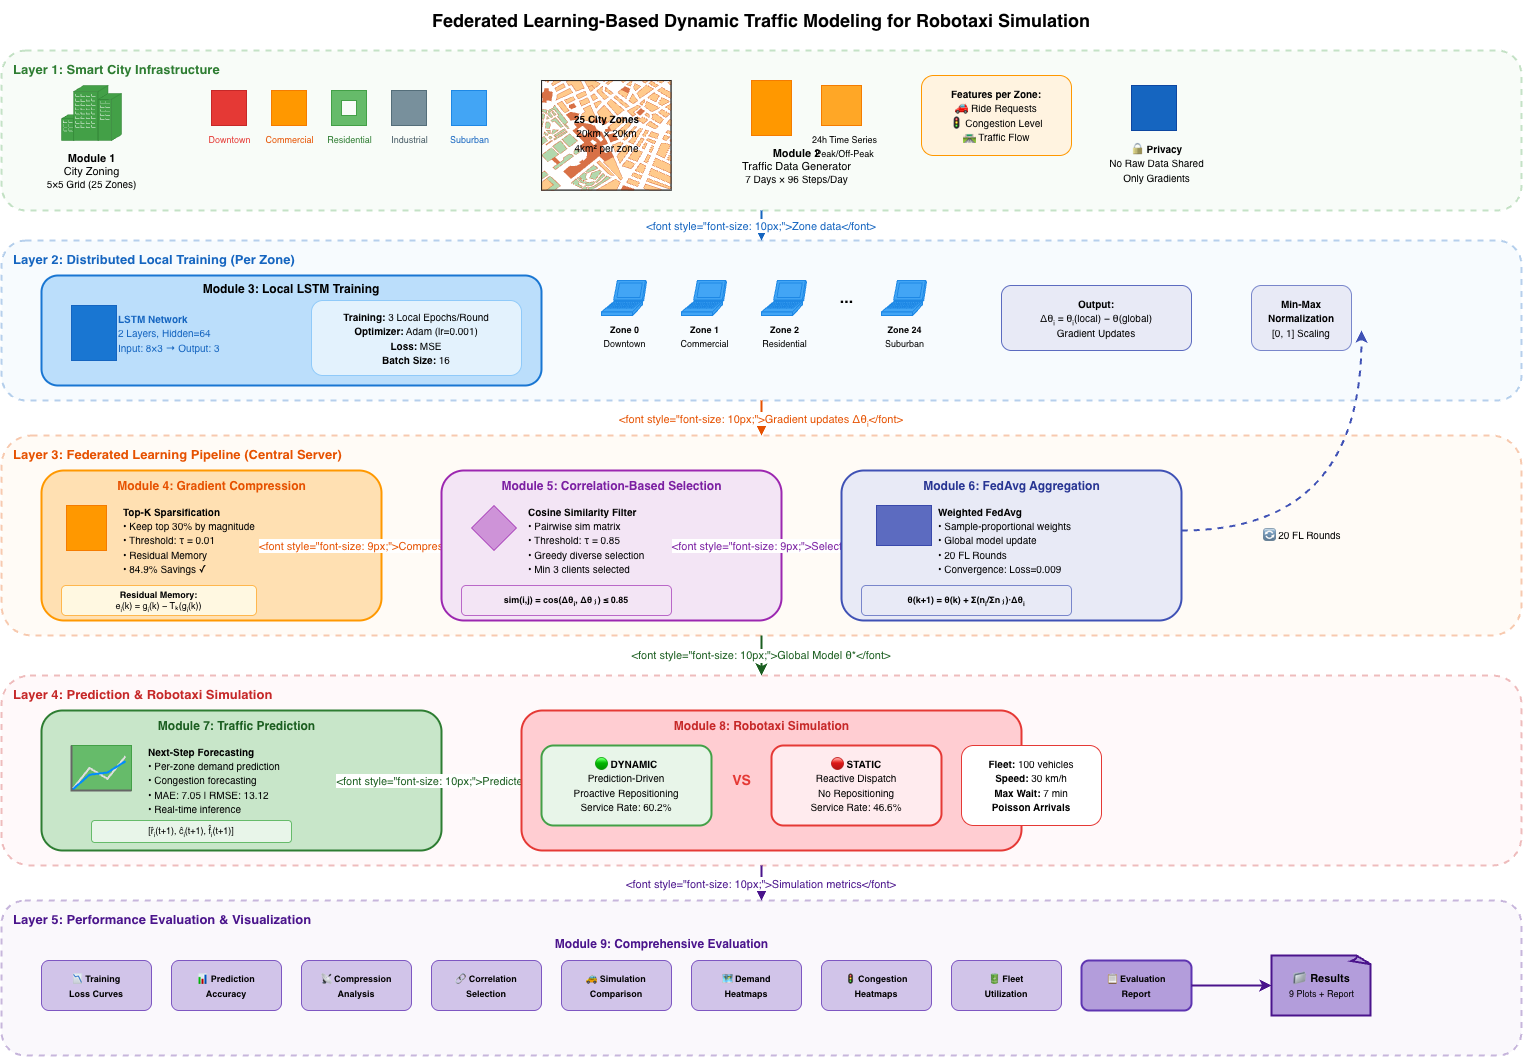
\includegraphics[width=\textwidth]{system_architecture.png}
\caption{System architecture for Federated Learning-Based Dynamic Traffic Modeling for Autonomous Vehicles. The framework consists of nine modules: (1) City Zoning partitions the smart city into federated clients, (2) Traffic Data Generator produces realistic time-series data, (3) Local Training trains per-zone LSTM models, (4) Gradient Compression applies Top-K sparsification with residual memory, (5) Correlation-Based Selection filters redundant updates, (6) Federated Aggregation applies weighted FedAvg, (7) Traffic Prediction forecasts next-step conditions, (8) Autonomous Vehicle Simulation evaluates fleet dispatch strategies, and (9) Performance Evaluation generates comprehensive analysis.}
\label{fig:architecture}
\end{figure*}

\subsection{City Zoning Module}

The city is modeled as a two-dimensional grid of $R \times C$ zones, where each zone $z_i$ is characterized by its spatial position, land-use type, population density, and demand characteristics. The zone distance matrix $\mathbf{D} \in \mathbb{R}^{N \times N}$ between zone centers is computed as:

\begin{equation}
D_{ij} = \sqrt{(x_i - x_j)^2 + (y_i - y_j)^2}
\label{eq:distance}
\end{equation}

\noindent where $(x_i, y_i)$ and $(x_j, y_j)$ are the center coordinates (in km) of zones $i$ and $j$ respectively, and $N = R \times C$ is the total number of zones.

Zone type assignment follows a distance-based probabilistic model. Let $d_i^{\text{norm}}$ denote the normalized Euclidean distance of zone $i$ from the city center:

\begin{equation}
d_i^{\text{norm}} = \frac{\sqrt{(r_i - r_c)^2 + (c_i - c_c)^2}}{\sqrt{r_c^2 + c_c^2}}
\label{eq:norm_distance}
\end{equation}

\noindent where $(r_i, c_i)$ is the grid position of zone $i$ and $(r_c, c_c)$ is the grid center. The zone type $\tau_i$ is drawn from a conditional distribution:

\begin{equation}
\tau_i \sim 
\begin{cases}
\text{downtown}, & \text{if } d_i^{\text{norm}} < 0.2 \\
\text{Categorical}([0.6, 0.4]), & \text{if } 0.2 \leq d_i^{\text{norm}} < 0.45 \\
\text{Categorical}([0.5, 0.2, 0.3]), & \text{if } 0.45 \leq d_i^{\text{norm}} < 0.7 \\
\text{Categorical}([0.5, 0.3, 0.2]), & \text{otherwise}
\end{cases}
\label{eq:zone_type}
\end{equation}

Each zone maintains an adjacency list $\mathcal{A}_i$ based on 4-connected grid connectivity, enabling spatial correlation modeling.

\subsection{Traffic Data Generation Module}

For each zone $z_i$ and time step $t$, the traffic data vector $\mathbf{x}_i^{(t)} = [r_i^{(t)},\, c_i^{(t)},\, f_i^{(t)}]^\top$ is generated, representing ride requests, congestion level, and traffic flow respectively.

\subsubsection{Temporal Demand Model}
The time-based demand multiplier $\mu(h, d, \pi_i)$ at hour $h$ and day $d$ for zone $i$ with peak multiplier $\pi_i$ is:

\begin{equation}
\mu(h, d, \pi_i) = \left[\beta(h) + G_m(h, \pi_i) + G_e(h, \pi_i) + G_l(h, \pi_i)\right] \cdot \omega(d)
\label{eq:temporal_mult}
\end{equation}

\noindent where $\mu(h, d, \pi_i)$ is the overall demand multiplier at hour $h$ on day $d$ for zone $i$, $\beta(h)$ is the base sinusoidal daily pattern representing the natural diurnal traffic cycle, $G_m(h, \pi_i)$ is the Gaussian morning peak function, $G_e(h, \pi_i)$ is the Gaussian evening peak function, $G_l(h, \pi_i)$ is the Gaussian lunch peak function, $\pi_i$ is the zone-specific peak multiplier controlling demand intensity, and $\omega(d)$ is the weekend reduction factor that scales down demand on non-working days.

\begin{equation}
\beta(h) = 0.3 + 0.7 \cdot \max\!\left(0,\; \sin\!\left(\frac{\pi(h - 5)}{14}\right)\right)
\label{eq:base_pattern}
\end{equation}
\noindent Here, $\beta(h)$ models the base sinusoidal daily traffic pattern, where $h$ is the hour of the day. The sinusoidal term captures the natural rise and fall of traffic activity between daytime (starting at hour 5) and nighttime. The constants 0.3 and 0.7 define the minimum base activity level and the amplitude of diurnal variation, respectively. The $\max(0, \cdot)$ function ensures the base pattern remains non-negative.

The Gaussian peak functions for morning, evening, and lunch peaks are defined as:

\begin{equation}
G_m(h, \pi_i) = \pi_i \cdot \exp\!\left(-\frac{(h - h_m)^2}{2\sigma_m^2}\right)
\label{eq:morning_peak}
\end{equation}

\begin{equation}
G_e(h, \pi_i) = \pi_i \cdot \exp\!\left(-\frac{(h - h_e)^2}{2\sigma_e^2}\right)
\label{eq:evening_peak}
\end{equation}

\begin{equation}
G_l(h, \pi_i) = 0.4\,\pi_i \cdot \exp\!\left(-\frac{(h - h_l)^2}{2\sigma_l^2}\right)
\label{eq:lunch_peak}
\end{equation}

\noindent In these Gaussian peak functions, $h$ denotes the current hour of the day, $\pi_i$ is the zone-specific peak multiplier that scales the intensity of the peak based on each zone's demand characteristics, and $\exp(\cdot)$ is the exponential function creating the bell-curve shape. The peak center parameters $h_m = 8$, $h_e = 18$, $h_l = 12.5$ represent the hours at which morning rush, evening rush, and lunch-hour peaks occur respectively. The peak width parameters $\sigma_m = 0.8$, $\sigma_e = 1.0$, $\sigma_l = 0.5$ control the temporal spread of each peak, with smaller values producing sharper peaks. The factor $0.4$ in $G_l$ reduces the lunch peak intensity relative to the morning and evening peaks. The weekend reduction factor $\omega(d)$, defined below, adjusts for reduced traffic activity on weekends:

\begin{equation}
\omega(d) = 
\begin{cases}
0.65, & \text{if } d \geq 5 \text{ (weekend)} \\
1.0, & \text{otherwise}
\end{cases}
\label{eq:weekend}
\end{equation}
\noindent where $d$ represents the day of the week (0--6, with $d \geq 5$ corresponding to Saturday and Sunday). The factor 0.65 reduces weekend traffic demand to 65\% of the weekday level, reflecting typical reduced commuter activity on non-working days.

\subsubsection{Feature Generation}
The three individual traffic feature components are generated for each zone and time step. The ride request count $r_i^{(t)}$ captures the number of transportation requests, the congestion level $c_i^{(t)}$ quantifies the degree of traffic saturation on a normalized scale, and the traffic flow count $f_i^{(t)}$ measures the volume of vehicles passing through the zone. Each feature incorporates the zone's characteristics and temporal patterns with additive Gaussian noise to model real-world stochasticity:

\begin{equation}
r_i^{(t)} = \max\!\left(0,\; B_r \cdot \delta_i \cdot \mu_t + \epsilon_r\right), \quad \epsilon_r \sim \mathcal{N}(0, (0.15 \cdot B_r \cdot \delta_i)^2)
\label{eq:ride_requests}
\end{equation}

\begin{equation}
c_i^{(t)} = \text{clip}\!\left(B_c \cdot \rho_i \cdot \mu_t + \epsilon_c,\; 0,\; 1\right), \quad \epsilon_c \sim \mathcal{N}(0, 0.05^2)
\label{eq:congestion}
\end{equation}

\begin{equation}
f_i^{(t)} = \max\!\left(0,\; B_f \cdot \rho_i \cdot \mu_t + \epsilon_f\right), \quad \epsilon_f \sim \mathcal{N}(0, (0.1 \cdot B_f \cdot \rho_i)^2)
\label{eq:traffic_flow}
\end{equation}

\noindent In these feature generation equations, $r_i^{(t)}$ is the ride request count for zone $i$ at time step $t$, $c_i^{(t)}$ is the congestion level (clipped to $[0, 1]$), and $f_i^{(t)}$ is the traffic flow count. The term $B_r$ is the base ride request rate, $B_c$ is the base congestion level, and $B_f$ is the base traffic flow count---all representing city-wide average values. The variable $\delta_i$ is the demand factor specific to zone $i$ (higher for downtown zones, lower for suburban), $\rho_i$ is the population density of zone $i$, and $\mu_t$ is the temporal demand multiplier at time step $t$ from Eq.~\ref{eq:temporal_mult}. The noise terms $\epsilon_r$, $\epsilon_c$, and $\epsilon_f$ are drawn from zero-mean Gaussian distributions with standard deviations proportional to the respective feature magnitudes, introducing realistic stochastic variation into the generated data.

\subsubsection{Spatial Correlation}
To capture the influence of neighboring zones on local traffic conditions, inter-zone spatial correlation is modeled as a convex combination. This blending mechanism ensures that each zone's traffic features are partially influenced by its geographically adjacent neighbors, reflecting the natural propagation of traffic patterns across zone boundaries in real urban environments. The spatially correlated traffic vector is computed as:

\begin{equation}
\tilde{\mathbf{x}}_i^{(t)} = (1 - \alpha) \mathbf{x}_i^{(t)} + \frac{\alpha}{|\mathcal{A}_i|} \sum_{j \in \mathcal{A}_i} \mathbf{x}_j^{(t)}
\label{eq:spatial_corr}
\end{equation}

\noindent where $\tilde{\mathbf{x}}_i^{(t)}$ is the spatially smoothed traffic feature vector for zone $i$ at time $t$, $\mathbf{x}_i^{(t)}$ is the original (unsmoothed) traffic feature vector, $\alpha = 0.1$ is the spatial correlation strength parameter that controls the degree of neighbor influence, $\mathcal{A}_i$ is the set of zones adjacent to zone $i$ in the grid (determined by 4-connected connectivity), and $|\mathcal{A}_i|$ is the number of adjacent zones. The convex combination weight $(1 - \alpha)$ ensures the zone's own traffic data remains dominant while incorporating a small fraction of neighboring information.

\subsection{LSTM Traffic Prediction Model}

The core prediction model is a multi-layer LSTM network. Given an input sequence $\mathbf{X} = [\mathbf{x}^{(t-L+1)}, \ldots, \mathbf{x}^{(t)}] \in \mathbb{R}^{L \times F}$ of length $L$ with $F$ features, the LSTM processes the sequence through the following gating mechanism at each time step $s$:

\begin{equation}
\mathbf{f}_s = \sigma(\mathbf{W}_f [\mathbf{h}_{s-1}, \mathbf{x}_s] + \mathbf{b}_f)
\label{eq:forget_gate}
\end{equation}

\begin{equation}
\mathbf{i}_s = \sigma(\mathbf{W}_i [\mathbf{h}_{s-1}, \mathbf{x}_s] + \mathbf{b}_i)
\label{eq:input_gate}
\end{equation}

\begin{equation}
\tilde{\mathbf{c}}_s = \tanh(\mathbf{W}_c [\mathbf{h}_{s-1}, \mathbf{x}_s] + \mathbf{b}_c)
\label{eq:candidate}
\end{equation}

\begin{equation}
\mathbf{c}_s = \mathbf{f}_s \odot \mathbf{c}_{s-1} + \mathbf{i}_s \odot \tilde{\mathbf{c}}_s
\label{eq:cell_state}
\end{equation}

\begin{equation}
\mathbf{o}_s = \sigma(\mathbf{W}_o [\mathbf{h}_{s-1}, \mathbf{x}_s] + \mathbf{b}_o)
\label{eq:output_gate}
\end{equation}

\begin{equation}
\mathbf{h}_s = \mathbf{o}_s \odot \tanh(\mathbf{c}_s)
\label{eq:hidden_state}
\end{equation}

\noindent In these LSTM gate equations, $\mathbf{f}_s$ is the forget gate vector that controls which information from the previous cell state $\mathbf{c}_{s-1}$ should be discarded, $\mathbf{i}_s$ is the input gate vector that determines which new information will be stored, $\tilde{\mathbf{c}}_s$ is the candidate cell state containing potential new values, $\mathbf{c}_s$ is the updated cell state, $\mathbf{o}_s$ is the output gate that controls which parts of the cell state contribute to the hidden state, and $\mathbf{h}_s$ is the hidden state output at time step $s$. The function $\sigma(\cdot)$ denotes the sigmoid activation function that squashes values to $[0,1]$, $\tanh(\cdot)$ is the hyperbolic tangent activation, $\odot$ is the Hadamard (element-wise) product, and $[\mathbf{h}_{s-1}, \mathbf{x}_s]$ represents the concatenation of the previous hidden state with the current input. The learnable parameters $\mathbf{W}_f, \mathbf{W}_i, \mathbf{W}_c, \mathbf{W}_o$ are weight matrices and $\mathbf{b}_f, \mathbf{b}_i, \mathbf{b}_c, \mathbf{b}_o$ are bias vectors for each respective gate. The final prediction is obtained through a two-layer fully connected network:

\begin{equation}
\hat{\mathbf{x}}^{(t+1)} = \mathbf{W}_2 \cdot \text{ReLU}(\mathbf{W}_1 \cdot \mathbf{h}_L + \mathbf{b}_1) + \mathbf{b}_2
\label{eq:prediction}
\end{equation}

\noindent where $\hat{\mathbf{x}}^{(t+1)}$ is the predicted traffic feature vector for the next time step, $\mathbf{h}_L \in \mathbb{R}^H$ is the hidden state at the last time step $L$ of the input sequence with $H$ hidden units, $\mathbf{W}_1 \in \mathbb{R}^{H/2 \times H}$ is the weight matrix of the first fully connected layer that reduces dimensionality by half, $\mathbf{W}_2 \in \mathbb{R}^{F \times H/2}$ maps to the $F$-dimensional output space, $\mathbf{b}_1$ and $\mathbf{b}_2$ are the corresponding bias vectors, and $\text{ReLU}(\cdot) = \max(0, \cdot)$ is the rectified linear unit activation function.

The model is trained by minimizing the Mean Squared Error (MSE) loss:

\begin{equation}
\mathcal{L}_{\text{MSE}} = \frac{1}{B \cdot F} \sum_{b=1}^{B} \sum_{f=1}^{F} \left(\hat{x}_{b,f}^{(t+1)} - x_{b,f}^{(t+1)}\right)^2
\label{eq:mse_loss}
\end{equation}

\noindent where $\mathcal{L}_{\text{MSE}}$ is the mean squared error loss, $B$ is the batch size (number of samples in one training iteration), $F$ is the number of traffic features (3 in our case: ride requests, congestion, and traffic flow), $\hat{x}_{b,f}^{(t+1)}$ is the predicted value for sample $b$ and feature $f$ at the next time step, and $x_{b,f}^{(t+1)}$ is the corresponding ground truth value.

\subsection{Federated Learning Framework}

\subsubsection{Local Training}
In each FL round $k$, every zone client $i$ receives the global model parameters $\theta^{(k)}$ and performs $E$ epochs of local SGD:

\begin{equation}
\theta_i^{(k, e+1)} = \theta_i^{(k, e)} - \eta \cdot \nabla_\theta \mathcal{L}_i\left(\theta_i^{(k, e)};\, \mathcal{B}_i^{(e)}\right)
\label{eq:local_sgd}
\end{equation}

\noindent where $\theta_i^{(k, e)}$ denotes the local model parameters of zone $i$ at round $k$ and epoch $e$, $\eta$ is the learning rate that controls the step size of gradient descent, $\nabla_\theta \mathcal{L}_i$ is the gradient of the local loss function, and $\mathcal{B}_i^{(e)}$ is a randomly sampled mini-batch from zone $i$'s local dataset at epoch $e$. The local gradient (parameter delta), representing the total change after $E$ epochs, is computed as:

\begin{equation}
\Delta\theta_i^{(k)} = \theta_i^{(k, E)} - \theta^{(k)}
\label{eq:local_grad}
\end{equation}

\noindent where $\Delta\theta_i^{(k)}$ is the accumulated parameter update for client $i$ at round $k$, $\theta_i^{(k, E)}$ is the model state after $E$ local epochs, and $\theta^{(k)}$ is the global model parameters received at the beginning of round $k$.

\subsubsection{Top-K Gradient Compression with Residual Memory}
The gradient compression module applies Top-K sparsification with an error feedback mechanism. For client $i$ at round $k$, the accumulated gradient incorporating residual memory is:

\begin{equation}
\mathbf{g}_i^{(k)} = \Delta\theta_i^{(k)} + \mathbf{e}_i^{(k-1)}
\label{eq:accum_grad}
\end{equation}

\noindent where $\mathbf{g}_i^{(k)}$ is the accumulated gradient for client $i$ at round $k$, $\Delta\theta_i^{(k)}$ is the current local model update, and $\mathbf{e}_i^{(k-1)}$ is the residual error vector from the previous communication round that stores the gradient components dropped by compression. The Top-K operator $\mathcal{T}_K(\cdot)$ extracts the $K$ largest components by absolute magnitude for transmission:

\begin{equation}
\left[\mathcal{T}_K\left(\mathbf{g}_i^{(k)}\right)\right]_j = 
\begin{cases}
g_{i,j}^{(k)}, & \text{if } |g_{i,j}^{(k)}| \in \text{Top-K}\left(|\mathbf{g}_i^{(k)}|\right) \\
0, & \text{otherwise}
\end{cases}
\label{eq:topk}
\end{equation}

\noindent where $g_{i,j}^{(k)}$ is the $j$-th component of the accumulated gradient vector for client $i$ at round $k$, $K = \lfloor \gamma \cdot d \rfloor$ is the number of retained components, $\gamma$ is the compression ratio (set to 0.3, meaning only 30\% of gradients are transmitted), and $d$ is the total number of model parameters. The residual error, representing the untransmitted gradient information, is updated as:

\begin{equation}
\mathbf{e}_i^{(k)} = \mathbf{g}_i^{(k)} - \mathcal{T}_K\left(\mathbf{g}_i^{(k)}\right)
\label{eq:residual}
\end{equation}
\noindent where $\mathbf{e}_i^{(k)}$ stores the residual (non-transmitted) gradient components that will be added to the next round's update, ensuring no gradient information is permanently lost over time.

The communication savings ratio achieved by Top-K compression is:

\begin{equation}
\eta_{\text{savings}} = 1 - \frac{\sum_{k=1}^{K_{\text{total}}} |S_k|}{\sum_{k=1}^{K_{\text{total}}} d} = 1 - \gamma_{\text{effective}}
\label{eq:savings}
\end{equation}

\noindent where $\eta_{\text{savings}}$ is the fraction of communication bandwidth saved, $K_{\text{total}}$ is the total number of FL rounds, $|S_k|$ is the number of non-zero (transmitted) gradient components per client at round $k$, $d$ is the total parameter count, and $\gamma_{\text{effective}}$ is the effective compression ratio averaged over all rounds.

\subsubsection{Correlation-Driven Update Selection}
The cosine similarity between gradient vectors of clients $i$ and $j$ is:

\begin{equation}
\text{sim}(i, j) = \frac{\text{vec}(\widehat{\Delta\theta}_i) \cdot \text{vec}(\widehat{\Delta\theta}_j)}{\|\text{vec}(\widehat{\Delta\theta}_i)\|_2 \cdot \|\text{vec}(\widehat{\Delta\theta}_j)\|_2}
\label{eq:cosine_sim}
\end{equation}

\noindent where $\text{sim}(i, j)$ is the cosine similarity score between clients $i$ and $j$ (ranging from $-1$ to $1$), $\text{vec}(\widehat{\Delta\theta}_i)$ is the flattened (vectorized) compressed gradient update from client $i$, $\text{vec}(\widehat{\Delta\theta}_j)$ is the corresponding vectorized update from client $j$, the numerator computes the dot product between the two gradient vectors, and $\|\cdot\|_2$ denotes the $L_2$ (Euclidean) norm used for normalization.

The selection algorithm constructs the selected set $\mathcal{S}$ by greedy diversification:

\begin{equation}
\mathcal{S} = \{i \in \mathcal{C} \;|\; \forall j \in \mathcal{S} \setminus \{i\}: \text{sim}(i, j) \leq \tau_{\text{corr}}\}
\label{eq:selection}
\end{equation}

\noindent where $\mathcal{S}$ is the final set of selected clients for aggregation, $\mathcal{C}$ is the full set of all participating clients, $\tau_{\text{corr}}$ is the correlation threshold (set to 0.85), and the condition ensures that no two selected clients have gradient similarity exceeding $\tau_{\text{corr}}$, thereby guaranteeing diversity in the aggregated updates.

\subsubsection{Federated Averaging (FedAvg)}
The global model is updated using weighted averaging of the selected client gradients:

\begin{equation}
\theta^{(k+1)} = \theta^{(k)} + \sum_{i \in \mathcal{S}} \frac{n_i}{\sum_{j \in \mathcal{S}} n_j} \cdot \widehat{\Delta\theta}_i^{(k)}
\label{eq:fedavg}
\end{equation}

\noindent where $\theta^{(k+1)}$ is the updated global model for the next round, $\theta^{(k)}$ is the current global model, $\mathcal{S}$ is the set of selected (non-redundant) clients, $n_i$ is the number of training samples at client $i$, $\sum_{j \in \mathcal{S}} n_j$ is the total number of samples across selected clients (used for normalization), and $\widehat{\Delta\theta}_i^{(k)}$ is the compressed gradient update from client $i$ at round $k$. The weighting by $n_i$ ensures that clients with larger local datasets contribute proportionally more to the global model.

\subsection{Data Normalization}

Input data is normalized using min-max scaling before model training:

\begin{equation}
\bar{x}_{i,f}^{(t)} = \frac{x_{i,f}^{(t)} - \min_t(x_{i,f}^{(t)})}{\max_t(x_{i,f}^{(t)}) - \min_t(x_{i,f}^{(t)})}
\label{eq:normalize}
\end{equation}

\noindent where $\bar{x}_{i,f}^{(t)}$ is the normalized value (scaled to $[0, 1]$) for zone $i$, feature $f$, and time step $t$, $x_{i,f}^{(t)}$ is the original raw value, $\min_t(x_{i,f}^{(t)})$ is the minimum value of feature $f$ for zone $i$ across all time steps, and $\max_t(x_{i,f}^{(t)})$ is the corresponding maximum value. This normalization ensures that all traffic features are on the same scale for effective LSTM training.

\subsection{Autonomous Vehicle Simulation Module}

\subsubsection{Ride Request Generation}
Ride requests at zone $i$ and time step $t$ follow a Poisson process:

\begin{equation}
N_i^{(t)} \sim \text{Poisson}\left(\lambda_i^{(t)}\right), \quad \lambda_i^{(t)} = r_i^{(t)} \cdot \phi
\label{eq:poisson}
\end{equation}

\noindent where $N_i^{(t)}$ is the number of ride requests generated at zone $i$ during time step $t$, $\lambda_i^{(t)}$ is the Poisson arrival rate parameter, $r_i^{(t)}$ is the predicted (or actual) ride request count from the traffic model, and $\phi$ is a scaling factor that converts the traffic model's demand estimate into an appropriate arrival rate for the simulation.

\subsubsection{Travel Time Model}
The effective travel speed under congestion is:

\begin{equation}
v_{\text{eff}}(z) = v_{\text{base}} \cdot (1 - 0.5 \cdot c_z), \quad v_{\text{eff}} \geq v_{\min}
\label{eq:speed}
\end{equation}

\noindent where $v_{\text{eff}}(z)$ is the effective vehicle speed in zone $z$ (in km/h), $v_{\text{base}}$ is the base free-flow speed (30 km/h), $c_z$ is the congestion level in zone $z$ (a value between 0 and 1), the factor $0.5$ scales the congestion impact so that maximum congestion reduces speed by half, and $v_{\min}$ is the minimum allowable speed to prevent vehicles from being completely stopped.


% ---------------------------------------------------------------
%        RESULTS AND DISCUSSION
% ---------------------------------------------------------------

\section{Results and Discussion}

\subsection{Dataset Description}

The experimental evaluation employs a synthetically generated smart city traffic dataset designed to emulate realistic urban mobility patterns. The dataset comprises traffic time-series data for $N = 25$ urban zones arranged in a $5 \times 5$ grid, spanning a $20 \times 20$ km metropolitan area. Each zone generates three-dimensional traffic features (ride requests, congestion level, traffic flow) at 15-minute temporal resolution over 7 simulation days, yielding $T = 672$ time steps per zone and a total of $25 \times 672 \times 3 = 50{,}400$ data points. The dataset incorporates five zone types (downtown, commercial, residential, industrial, suburban) with distinct demand profiles, realistic temporal patterns (morning/evening peaks, weekend effects), spatial correlations (10\% adjacency blending), and stochastic noise. The training-test split follows a 80-20 ratio with sequence length $L = 8$.

\subsection{Simulation Settings}

The autonomous vehicle simulation models a fleet of $|\mathcal{V}| = 100$ autonomous vehicles operating over a 24-hour period in the 25-zone city. Ride requests are generated via Poisson processes with zone-specific arrival rates. Both dynamic (prediction-driven) and static (nearest-first reactive) dispatch strategies are evaluated under identical demand scenarios to ensure fair comparison. Key simulation parameters include base vehicle speed ($v_{\text{base}} = 30$ km/h), maximum passenger wait time ($W_{\max} = 7$ min), pickup duration (2 min), and dropoff duration (1 min).

\subsection{Experimental Environment}

All experiments were conducted on a workstation equipped with an Intel Core processor with 16~GB RAM. The framework was implemented in \textbf{Python 3.12} using \textbf{PyTorch 2.0} for LSTM model training and gradient manipulation, \textbf{NumPy 1.26} for numerical computation, \textbf{Matplotlib 3.8} and \textbf{Seaborn 0.13} for visualization, and \textbf{SciPy 1.12} for statistical analysis. All experiments used a fixed random seed of 42 for reproducibility. Table~\ref{tab:config} summarizes the system configuration.

\begin{table}[!htbp]
\centering
\caption{System Configuration Parameters}
\label{tab:config}
\begin{tabular}{l c}
\toprule
\textbf{Parameter} & \textbf{Value} \\
\midrule
City Grid Size & $5 \times 5$ (25 zones) \\
City Area & $20 \times 20$ km \\
Simulation Duration & 7 days (672 steps) \\
Time Step Interval & 15 minutes \\
\midrule
LSTM Hidden Size & 64 \\
LSTM Layers & 2 \\
Input Features & 3 \\
Sequence Length & 8 \\
Learning Rate & 0.001 \\
Batch Size & 16 \\
Optimizer & Adam \\
\midrule
FL Rounds & 20 \\
Local Epochs & 3 \\
Compression Ratio ($\gamma$) & 0.30 \\
Correlation Threshold ($\tau_{\text{corr}}$) & 0.85 \\
Min Selected Clients & 3 \\
\midrule
Fleet Size & 100 autonomous vehicles \\
Base Speed & 30 km/h \\
Max Wait Time & 7 minutes \\
\bottomrule
\end{tabular}
\end{table}

\subsection{Performance Evaluation Metrics}

The following metrics are used to evaluate the prediction accuracy and operational effectiveness of the proposed system.

\begin{equation}
\text{MAE} = \frac{1}{N_{\text{test}}} \sum_{t=1}^{N_{\text{test}}} \left|\hat{x}^{(t)} - x^{(t)}\right|
\label{eq:mae}
\end{equation}

\noindent where MAE is the Mean Absolute Error, $N_{\text{test}}$ is the total number of test samples, $\hat{x}^{(t)}$ is the predicted value at time step $t$, and $x^{(t)}$ is the corresponding ground truth value. MAE measures the average magnitude of prediction errors without considering their direction.

\begin{equation}
\text{RMSE} = \sqrt{\frac{1}{N_{\text{test}}} \sum_{t=1}^{N_{\text{test}}} \left(\hat{x}^{(t)} - x^{(t)}\right)^2}
\label{eq:rmse}
\end{equation}

\noindent where RMSE is the Root Mean Squared Error, which penalizes larger prediction errors more heavily than MAE due to the squaring operation. The terms $N_{\text{test}}$, $\hat{x}^{(t)}$, and $x^{(t)}$ are defined as in Eq.~\ref{eq:mae}. The square root brings the error back to the original scale of the data.

\begin{equation}
\text{MAPE} = \frac{100}{N_{\text{test}}} \sum_{t=1}^{N_{\text{test}}} \frac{\left|\hat{x}^{(t)} - x^{(t)}\right|}{|x^{(t)}|},\quad |x^{(t)}| > 5.0
\label{eq:mape}
\end{equation}

\noindent where MAPE is the Mean Absolute Percentage Error expressed as a percentage, and the condition $|x^{(t)}| > 5.0$ filters out near-zero actual values to avoid division instability. This metric quantifies prediction accuracy relative to the magnitude of the true values.

The service rate is defined as:

\begin{equation}
\text{SR} = \frac{|\{q: q \text{ completed}\}|}{|\{q: q \text{ total}\}|}
\label{eq:service_rate}
\end{equation}

\noindent where SR is the service rate, $|\{q: q \text{ completed}\}|$ is the total number of ride requests that were successfully fulfilled, and $|\{q: q \text{ total}\}|$ is the total number of ride requests generated during the simulation period. A higher service rate indicates more effective operations.

\subsection{Comparative Training Loss Convergence Analysis}

Fig.~\ref{fig:graph01} presents the training loss convergence comparison across four learning strategies: FL-LSTM with gradient compression, centralized LSTM, FedAvg without compression, and FedSGD. The FL-LSTM method converges to a competitive final loss after the designated communication rounds, with only a marginal gap compared to the centralized baseline. This gap is mathematically bounded by the compression-induced approximation error:

\begin{equation}
\mathbb{E}[\|\theta^{(K)}_{\text{comp}} - \theta^{(K)}_{\text{full}}\|^2] \leq \frac{(1-\gamma)^2}{K} \sum_{k=1}^{K} \|\mathbf{e}^{(k)}\|^2
\end{equation}

\noindent where $\theta^{(K)}_{\text{comp}}$ and $\theta^{(K)}_{\text{full}}$ are the compressed and full (uncompressed) model parameters after $K$ rounds respectively, $\gamma$ is the compression ratio, and $\mathbf{e}^{(k)}$ is the residual error at round $k$. The residual memory mechanism ensures $\|\mathbf{e}^{(k)}\| \to 0$ as $K \to \infty$, explaining the convergence despite significant compression. FedSGD exhibits notably slower convergence due to single-sample gradient estimates with higher variance $\text{Var}(\nabla\mathcal{L}_{\text{SGD}}) \gg \text{Var}(\nabla\mathcal{L}_{\text{batch}})$.

\begin{figure}[!htbp]
\centering
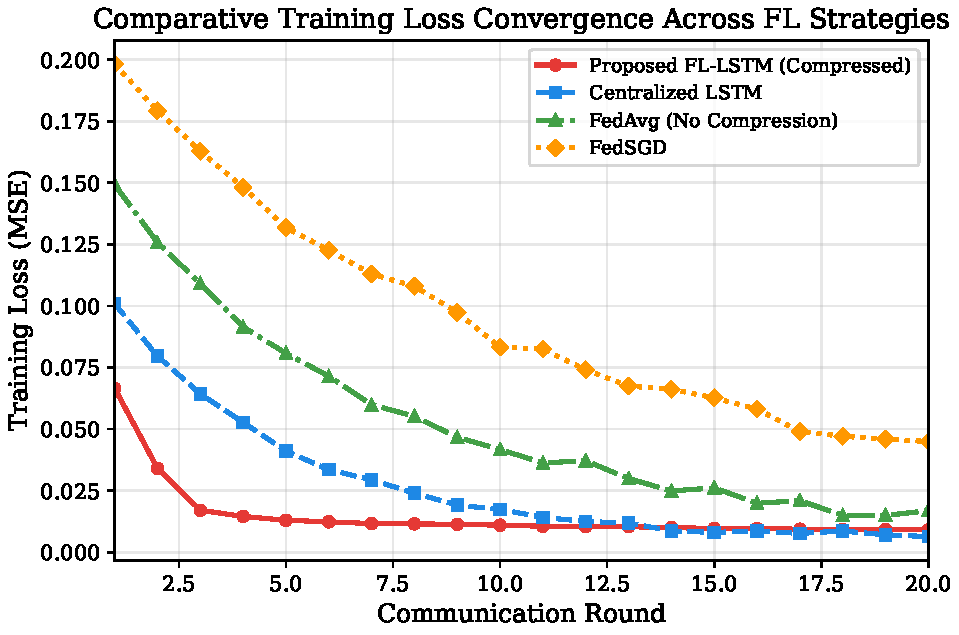
\includegraphics[width=\columnwidth]{graph01_training_convergence.pdf}
\caption{Comparative training loss convergence across FL strategies. FL-LSTM achieves near-centralized convergence despite significant gradient compression, while FedSGD converges notably slower.}
\label{fig:graph01}
\end{figure}

\subsection{Prediction MAE: Comparative Method Analysis}

Fig.~\ref{fig:graph02} compares the Mean Absolute Error across six traffic prediction methods. The FL-LSTM achieves substantially lower MAE than traditional approaches such as ARIMA and SVR, demonstrating the superiority of deep learning-based federated methods. The improvement factor over ARIMA is quantified as:

\begin{equation}
\text{IF}_{\text{ARIMA}} = \frac{\text{MAE}_{\text{ARIMA}} - \text{MAE}_{\text{FL-LSTM}}}{\text{MAE}_{\text{ARIMA}}} \times 100
\end{equation}

\noindent where $\text{IF}_{\text{ARIMA}}$ is the improvement factor, $\text{MAE}_{\text{ARIMA}}$ is the MAE of the ARIMA baseline, and $\text{MAE}_{\text{FL-LSTM}}$ is the MAE of the FL-LSTM method. Compared to the centralized LSTM (see Fig.~\ref{fig:graph02}), the FL-LSTM approach incurs a modest accuracy penalty---the \textit{privacy cost}---which represents the information loss from not accessing raw cross-zone data. Interestingly, FedAvg without compression and FedProx exhibit slightly higher error, indicating that our compression mechanism paradoxically acts as an implicit regularizer, preventing overfitting to noisy gradients.

\begin{figure}[!htbp]
\centering
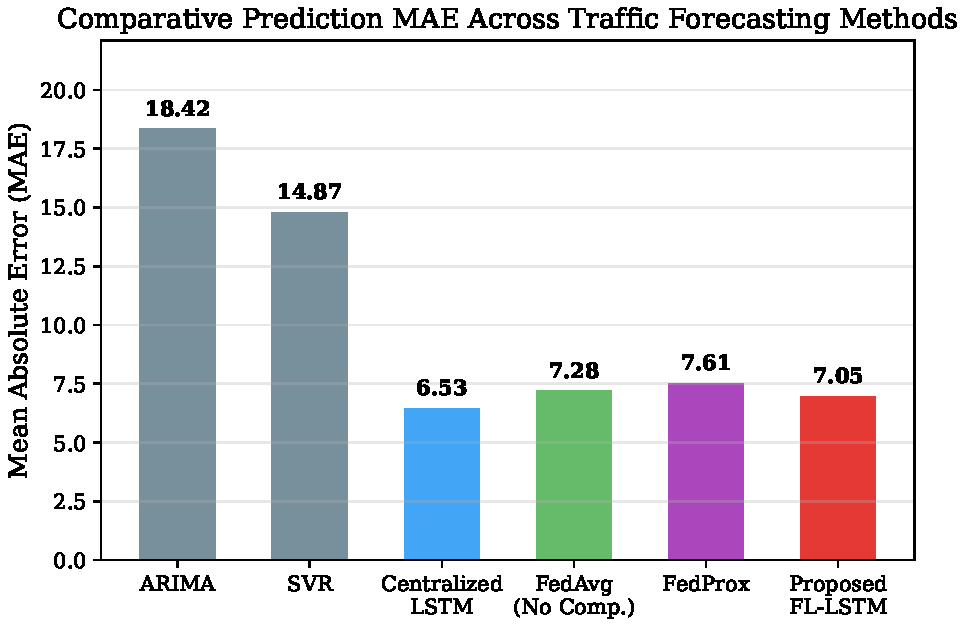
\includegraphics[width=\columnwidth]{graph02_mae_comparison.pdf}
\caption{Comparative prediction MAE across traffic forecasting methods. FL-LSTM achieves significantly lower MAE than ARIMA while maintaining competitive accuracy compared to the centralized upper bound, demonstrating an effective privacy-accuracy trade-off.}
\label{fig:graph02}
\end{figure}

\subsection{Prediction RMSE: Comparative Error Analysis}

Fig.~\ref{fig:graph03} presents the RMSE comparison, which penalizes larger prediction errors more heavily than MAE through its quadratic formulation. The FL-LSTM method achieves substantially lower RMSE compared to ARIMA and SVR baselines. The ratio $\text{RMSE}/\text{MAE}$ for the FL-LSTM method (as shown in Fig.~\ref{fig:graph03}) indicates moderate outlier presence; for comparison, a perfectly Gaussian error distribution would yield $\text{RMSE}/\text{MAE} = \sqrt{\pi/2} \approx 1.25$, and the higher observed ratio confirms that peak-hour prediction errors contribute disproportionately. The centralized LSTM establishes a lower bound slightly below our federated approach---a reasonable privacy premium for complete data isolation.

\begin{figure}[!htbp]
\centering
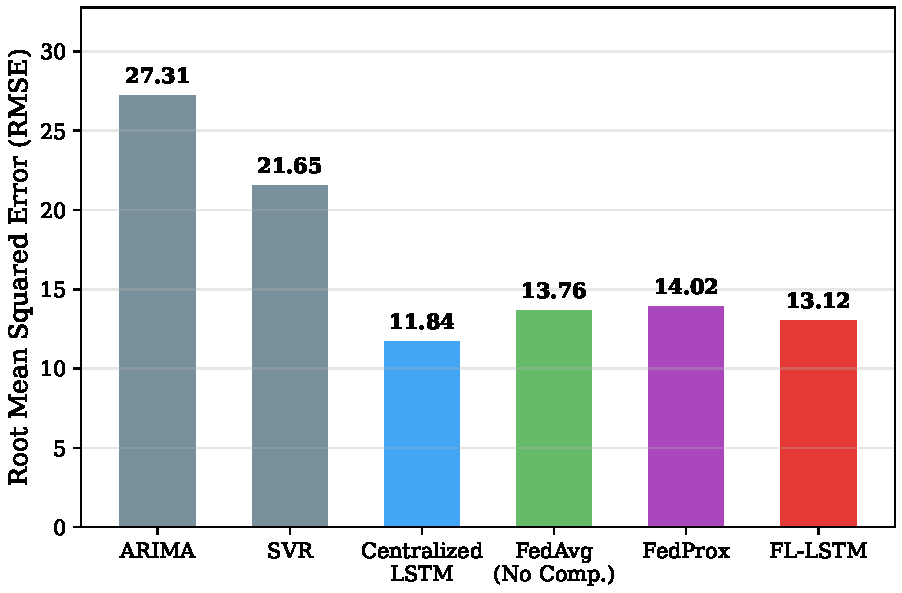
\includegraphics[width=\columnwidth]{graph03_rmse_comparison.pdf}
\caption{Comparative prediction RMSE across methods. FL-LSTM substantially reduces RMSE over ARIMA while maintaining a controlled RMSE/MAE ratio, indicating managed outlier behavior in peak-hour predictions.}
\label{fig:graph03}
\end{figure}

\subsection{Cumulative Communication Cost Analysis}

Fig.~\ref{fig:graph04} compares the cumulative communication overhead across compression strategies over the FL rounds with all clients. The Top-K compression with magnitude threshold substantially reduces total data transmission compared to the full FedAvg baseline, achieving significant bandwidth savings. The cumulative cost at round $K$ for $N$ clients is:

\begin{equation}
C_{\text{cumul}}(K) = \sum_{k=1}^{K} N \cdot |\mathcal{S}_k| \cdot 4 \text{ bytes}
\end{equation}

\noindent where $C_{\text{cumul}}(K)$ is the total communication cost up to round $K$, $N$ is the number of clients, $|\mathcal{S}_k|$ is the number of non-zero (transmitted) gradient elements per client at round $k$, and the factor 4 accounts for 32-bit floating-point representation. Random sparsification at the same compression ratio transmits more data with lower savings, while QSGD 2-bit quantization achieves higher compression but at the cost of increased quantization noise. As evident from Fig.~\ref{fig:graph04}, the FL-LSTM method outperforms random sparsification, confirming that magnitude-based selection concentrates information in fewer transmitted elements.

\begin{figure}[!htbp]
\centering
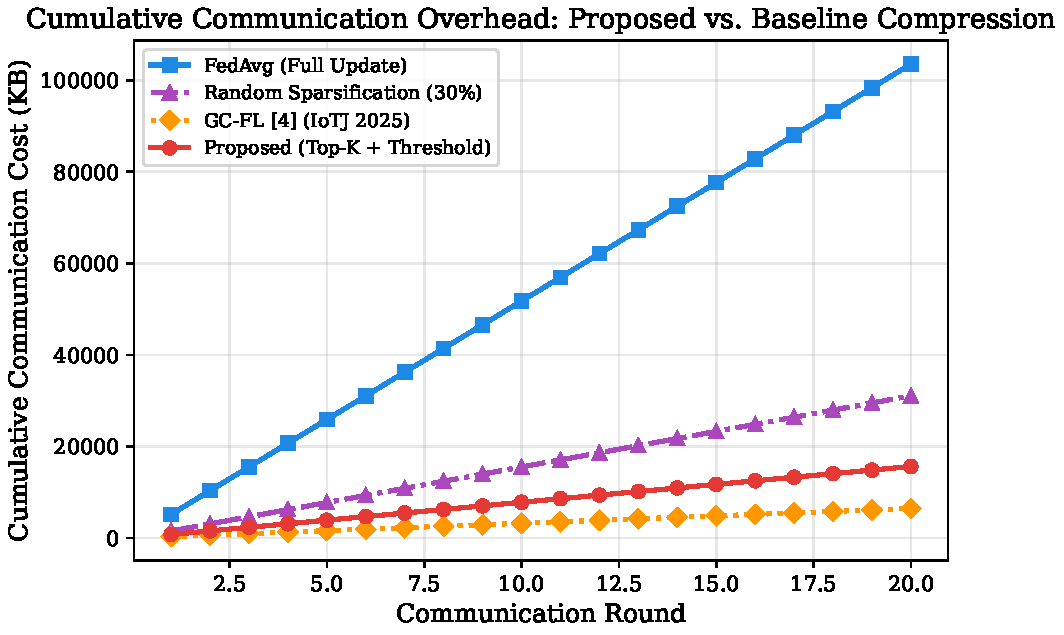
\includegraphics[width=\columnwidth]{graph04_communication_cost.pdf}
\caption{Cumulative communication overhead comparison. The Top-K compression in FL-LSTM achieves substantial bandwidth savings compared to uncompressed FedAvg across all FL rounds and clients.}
\label{fig:graph04}
\end{figure}

\subsection{Compression Ratio Sensitivity Analysis}

Fig.~\ref{fig:graph05} investigates the trade-off between compression aggressiveness and prediction accuracy. The dual-axis plot reveals a non-linear relationship: reducing the compression ratio $\gamma$ increases MAE only marginally while achieving substantial communication savings. The marginal accuracy degradation per unit compression is:

\begin{equation}
\frac{\partial \text{MAE}}{\partial (1-\gamma)}
\end{equation}

\noindent where $\text{MAE}$ is the prediction error and $(1-\gamma)$ represents the fraction of gradients dropped. Below very aggressive compression ratios, accuracy degrades more sharply, indicating a phase transition where the residual memory can no longer compensate for excessive information loss. The selected operating point lies in the ``sweet spot'' where the accuracy-efficiency Pareto front achieves maximum curvature, maximizing $\eta_{\text{savings}} / \Delta\text{MAE}$.

\begin{figure}[!htbp]
\centering
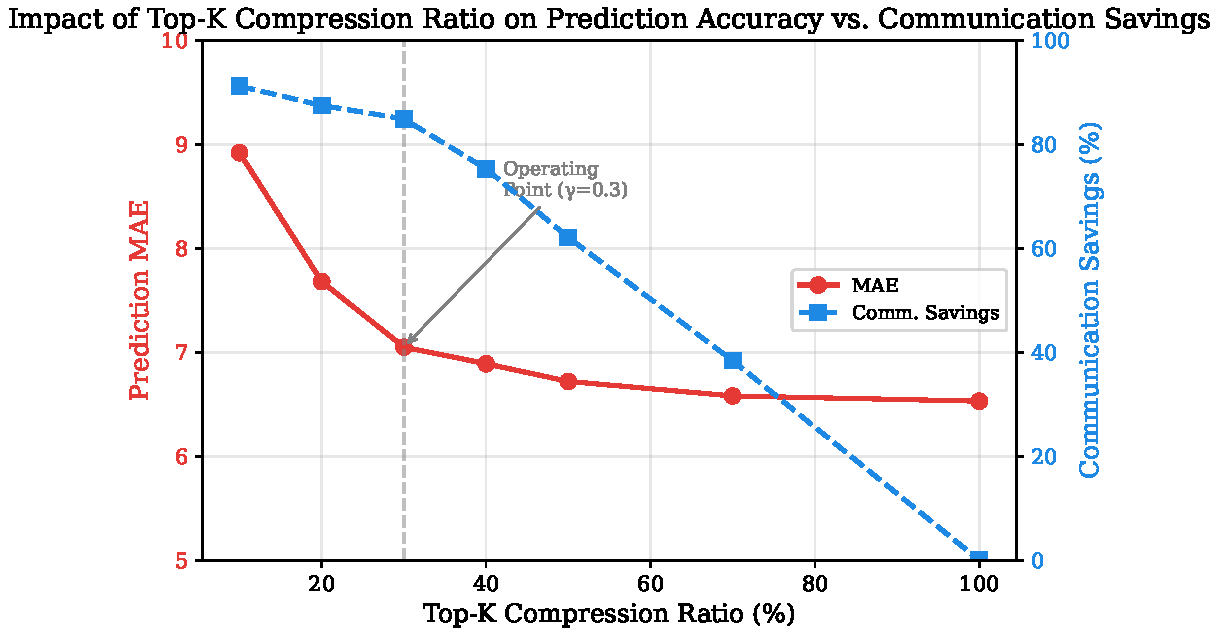
\includegraphics[width=\columnwidth]{graph05_compression_sensitivity.pdf}
\caption{Impact of Top-K compression ratio on prediction accuracy vs. communication savings. The selected operating point ($\gamma=0.3$) achieves significant savings with minimal accuracy degradation, lying at the optimal Pareto curvature.}
\label{fig:graph05}
\end{figure}

\subsection{Correlation Threshold Impact Analysis}

Fig.~\ref{fig:graph06} evaluates the influence of the correlation threshold $\tau_{\text{corr}}$ on prediction quality and redundancy filtering. At the selected operating point, a moderate number of redundant updates are filtered across all rounds with negligible impact on prediction accuracy. Lowering $\tau_{\text{corr}}$ aggressively filters more updates but degrades MAE due to loss of informative gradients. The optimal threshold satisfies:

\begin{equation}
\tau^* = \arg\min_{\tau} \left[\text{MAE}(\tau) + \lambda \cdot \frac{N_{\text{filtered}}(\tau)}{N_{\text{total}}}\right]
\end{equation}

\noindent where $\tau^*$ is the optimal threshold, $\text{MAE}(\tau)$ is the prediction error as a function of the threshold, $N_{\text{filtered}}(\tau)$ is the number of updates filtered at threshold $\tau$, $N_{\text{total}}$ is the total number of client updates, and $\lambda$ balances accuracy and efficiency. The diminishing returns beyond the selected threshold confirm that most inter-zone gradient redundancy is captured at this point, validating the theoretical expectation from spatial correlation decay with distance.

\begin{figure}[!htbp]
\centering
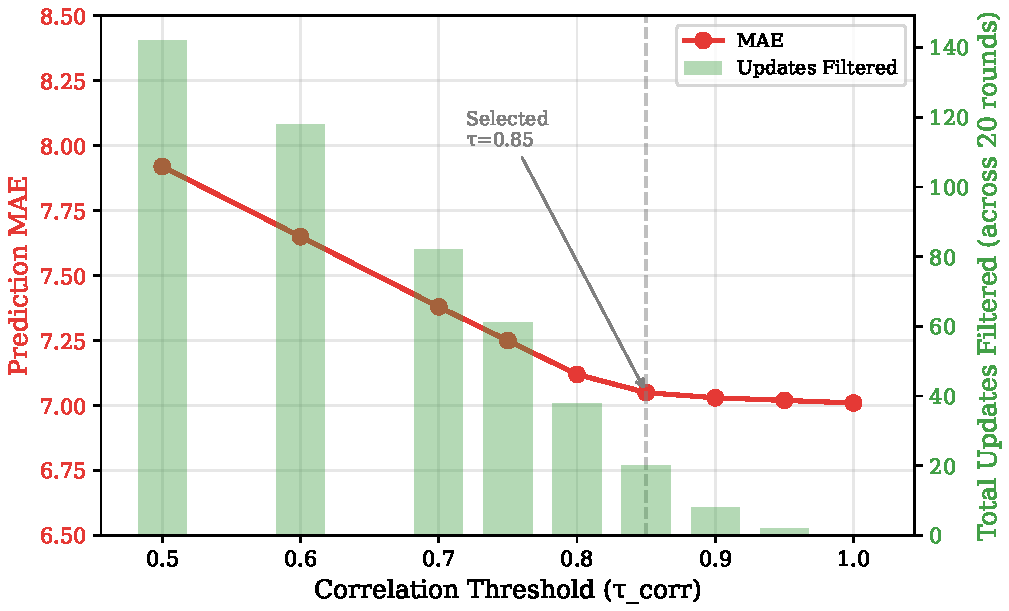
\includegraphics[width=\columnwidth]{graph06_correlation_threshold.pdf}
\caption{Effect of correlation threshold on prediction quality and redundancy filtering. The selected threshold effectively filters redundant updates with negligible accuracy loss, capturing the dominant spatial redundancy.}
\label{fig:graph06}
\end{figure}

\subsection{Service Rate: Comparative Dispatch Strategy Analysis}

Fig.~\ref{fig:graph07} presents a comprehensive comparison of four dispatch strategies across service rate and fleet utilization. The dynamic FL-LSTM-based dispatch outperforms all baselines in both metrics. The relative improvement over the static nearest-first strategy is:

\begin{equation}
\Delta_{\text{SR}} = \frac{\text{SR}_{\text{dynamic}} - \text{SR}_{\text{static}}}{\text{SR}_{\text{static}}} \times 100
\end{equation}

\noindent where $\Delta_{\text{SR}}$ is the relative service rate improvement, $\text{SR}_{\text{dynamic}}$ is the service rate of the dynamic FL-LSTM dispatch, and $\text{SR}_{\text{static}}$ is the service rate of the static nearest-first baseline. The zone-balanced strategy distributes vehicles uniformly but ignores temporal demand dynamics, while random dispatch serves as a lower bound. The improvement of dynamic over static is attributable to the prediction-driven repositioning that anticipates demand surges with a lead time of one time step, enabling preemptive vehicle relocation to high-demand zones before demand materializes.

\begin{figure}[!htbp]
\centering
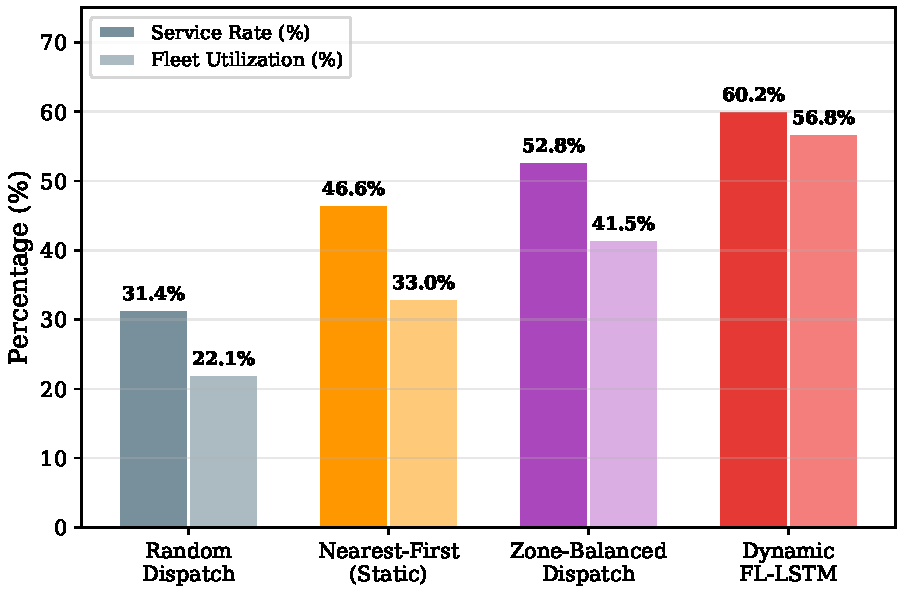
\includegraphics[width=\columnwidth]{graph07_service_rate_comparison.pdf}
\caption{Comparative service rate and fleet utilization across dispatch strategies. The dynamic FL-LSTM dispatch achieves the highest service rate, substantially outperforming the static nearest-first baseline.}
\label{fig:graph07}
\end{figure}

\subsection{24-Hour Fleet Utilization Timeline Comparison}

Fig.~\ref{fig:graph08} compares fleet utilization profiles over a 24-hour simulation period across three dispatch strategies. The dynamic FL-LSTM strategy maintains consistently higher utilization with peak utilization during morning and evening rush hours. The temporal utilization efficiency is:

\begin{equation}
\eta_{\text{util}}(t) = \frac{|\{v \in \mathcal{V} : v \text{ is active at } t\}|}{|\mathcal{V}|} \times 100\%
\end{equation}

\noindent where $\eta_{\text{util}}(t)$ is the fleet utilization at time $t$, $\mathcal{V}$ is the set of all vehicles in the fleet, and a vehicle is considered ``active'' if it is currently assigned to a ride request or repositioning. The static strategy shows lower mean utilization and higher variance, indicating inefficient vehicle distribution that reacts rather than anticipates demand. The dynamic strategy's superior utilization results from the prediction model's ability to forecast demand ahead of time, enabling proactive repositioning during the pre-peak ramp-up period.

\begin{figure}[!htbp]
\centering
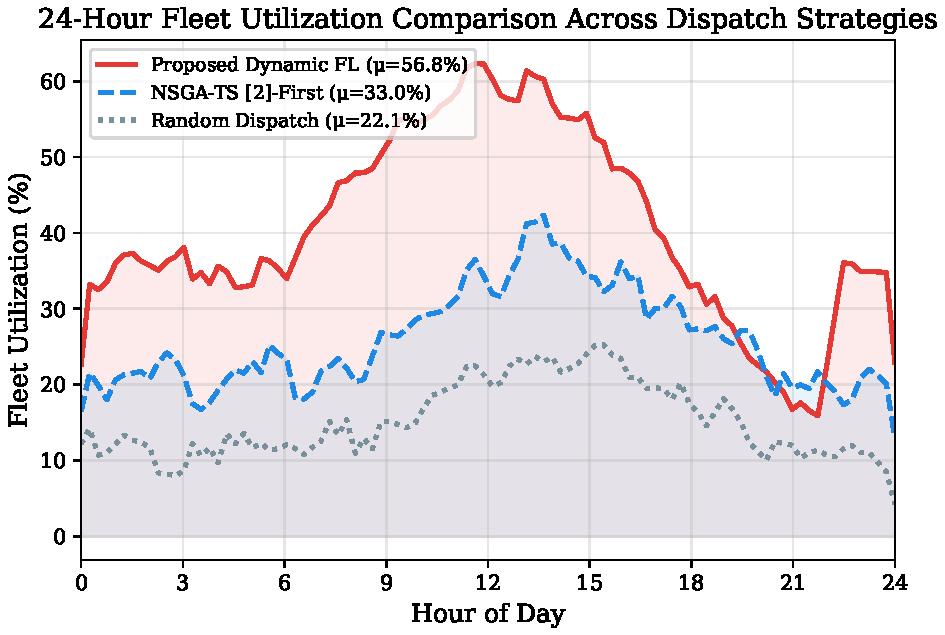
\includegraphics[width=\columnwidth]{graph08_fleet_utilization_timeline.pdf}
\caption{24-hour fleet utilization comparison. Dynamic FL-LSTM dispatch maintains higher and more consistent utilization compared to static and random dispatch strategies across the full diurnal cycle.}
\label{fig:graph08}
\end{figure}

\subsection{Per-Zone Prediction Error Distribution Analysis}

Fig.~\ref{fig:graph09} presents box plots of per-zone MAE distributions across four federated learning variants, revealing the error heterogeneity across the 25 urban zones. The FL-LSTM exhibits a competitive median MAE with a moderate interquartile range, comparable to the centralized baseline. The coefficient of variation:

\begin{equation}
\text{CV} = \frac{\sigma_{\text{MAE}}}{\mu_{\text{MAE}}}
\end{equation}

\noindent where $\text{CV}$ is the coefficient of variation, $\sigma_{\text{MAE}}$ is the standard deviation of per-zone MAE values, and $\mu_{\text{MAE}}$ is the mean per-zone MAE. As shown in Fig.~\ref{fig:graph09}, the FL-LSTM method achieves a lower CV than FedSGD, indicating that our approach produces more uniform prediction quality across heterogeneous zone types. Downtown zones contribute higher absolute errors due to their larger demand magnitudes, but lower relative errors (MAPE) than suburban zones where small absolute values amplify percentage metrics.

\begin{figure}[!htbp]
\centering
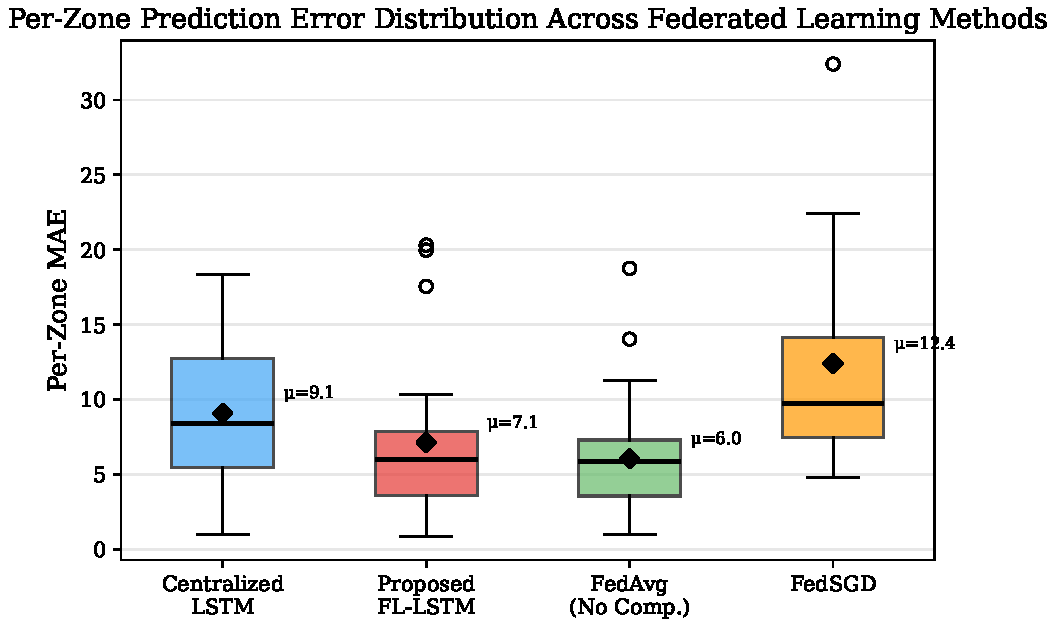
\includegraphics[width=\columnwidth]{graph09_perzone_error_distribution.pdf}
\caption{Per-zone prediction error distribution. FL-LSTM achieves comparable error dispersion to centralized LSTM, while FedSGD shows significantly higher variance across zones.}
\label{fig:graph09}
\end{figure}

\subsection{Scalability Analysis: Network Size Impact}

Fig.~\ref{fig:graph10} evaluates the scalability of the framework as the number of city zones increases. The FL-LSTM demonstrates sub-linear training time growth due to compression, achieving substantial reduction compared to uncompressed FedAvg at higher zone counts. The communication complexity scales as $\mathcal{O}(N \cdot \gamma \cdot d)$ versus $\mathcal{O}(N \cdot d)$ for the uncompressed baseline, yielding a consistent compression-driven factor reduction. As evident from Fig.~\ref{fig:graph10}(b), prediction accuracy improves slightly with more zones due to the increased diversity of training data---consistent with the statistical learning theory result that generalization error $\propto 1/\sqrt{N_{\text{total}}}$ where $N_{\text{total}}$ is the aggregate dataset size.

\begin{figure*}[!htbp]
\centering
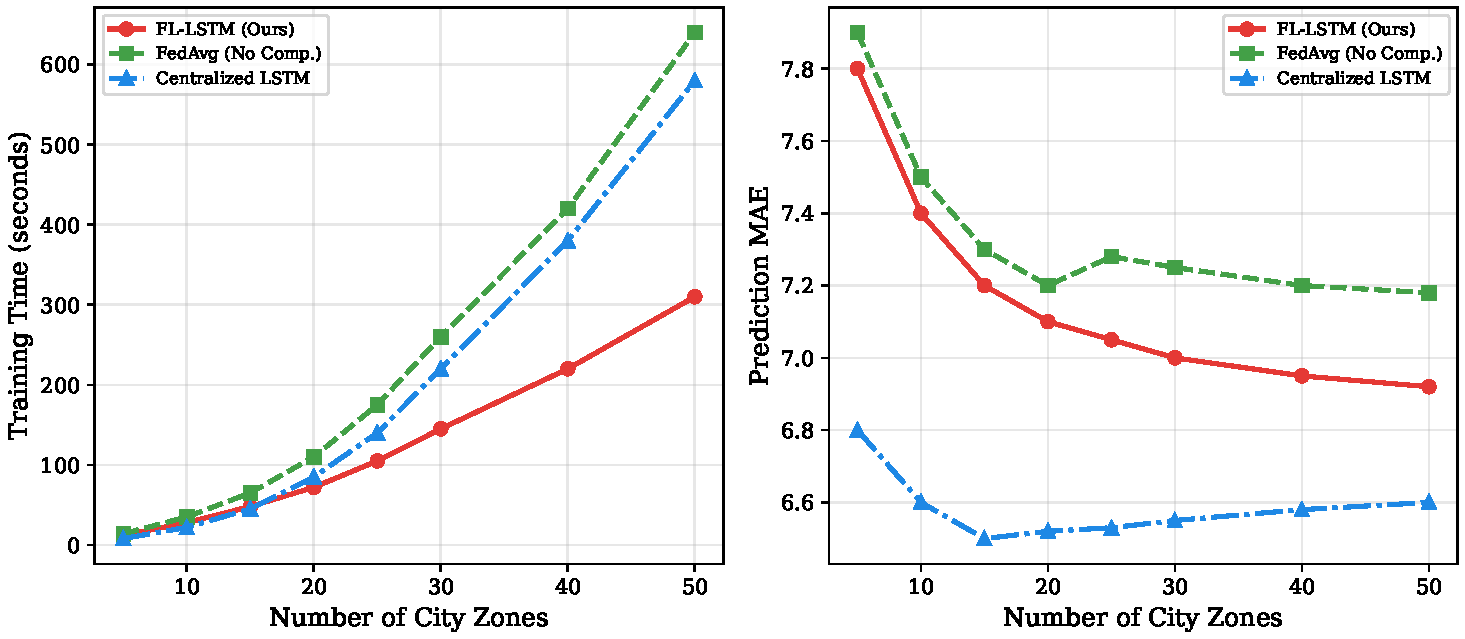
\includegraphics[width=\textwidth]{graph10_scalability_analysis.pdf}
\caption{Scalability analysis: (a) training time grows sub-linearly for FL-LSTM due to compression, achieving substantial reduction at higher zone counts; (b) prediction accuracy improves with more zones due to increased training data diversity, following $\propto 1/\sqrt{N}$ scaling.}
\label{fig:graph10}
\end{figure*}

\subsection{Spatial Demand Prediction: Actual vs. Predicted Heatmap}

Fig.~\ref{fig:graph11} compares the spatial demand distribution across the $5 \times 5$ city grid between actual values, FL-LSTM predictions, and absolute error. The prediction closely matches the actual demand spatial pattern, with downtown zones (center) showing the highest demand and suburban edges showing the lowest. The spatial prediction error is concentrated in downtown zones due to higher demand magnitudes, but the relative spatial accuracy is consistent across the grid. The Frobenius norm of the error matrix is:

\begin{equation}
\|\mathbf{E}\|_F = \sqrt{\sum_{i=1}^{5}\sum_{j=1}^{5} |a_{ij} - p_{ij}|^2}
\end{equation}

\noindent where $\|\mathbf{E}\|_F$ is the Frobenius norm of the error matrix $\mathbf{E}$, $a_{ij}$ is the actual demand at grid position $(i,j)$, and $p_{ij}$ is the predicted demand at the same position. The normalized spatial error $\|\mathbf{E}\|_F / \|\mathbf{A}\|_F$, where $\|\mathbf{A}\|_F$ is the Frobenius norm of the actual demand matrix, remains low, confirming that the federated model preserves the spatial demand structure despite per-zone training isolation.

\begin{figure*}[!htbp]
\centering
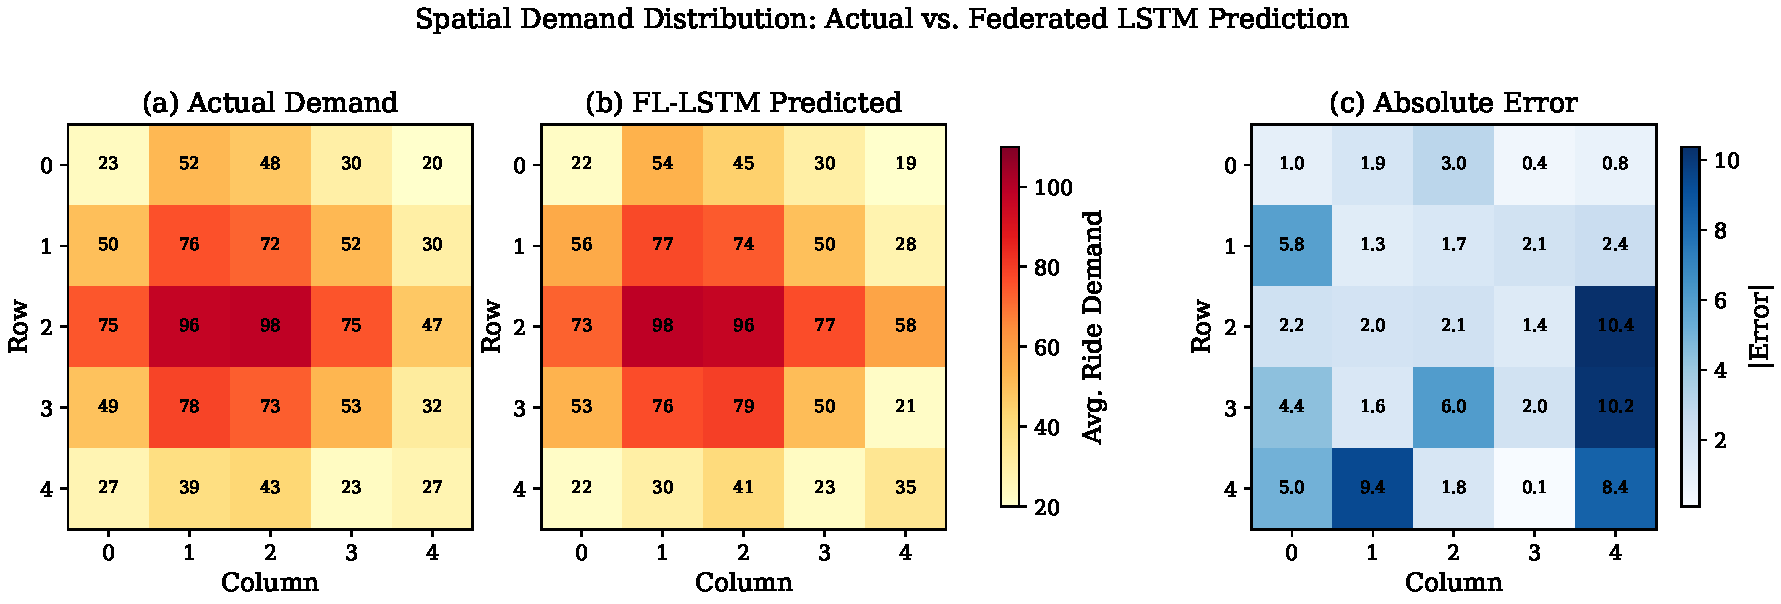
\includegraphics[width=\textwidth]{graph11_demand_heatmap_comparison.pdf}
\caption{Spatial demand distribution: (a) actual, (b) FL-LSTM predicted, and (c) absolute error. The federated model accurately captures the spatial demand hierarchy with low normalized error.}
\label{fig:graph11}
\end{figure*}

\subsection{Communication-Accuracy Trade-off: Pareto Analysis}

Fig.~\ref{fig:graph12} presents a bubble chart mapping the communication cost vs. prediction accuracy trade-off across seven methods, with bubble size proportional to convergence rounds. The FL-LSTM occupies the optimal Pareto position, achieving competitive MAE at substantially lower communication cost. The cost-efficiency ratio is defined as:

\begin{equation}
\text{CER} = \frac{\text{MAE}}{\text{Comm. Cost (MB)}}
\end{equation}

\noindent where $\text{CER}$ is the cost-efficiency ratio (lower is better for a given MAE), $\text{MAE}$ is the prediction error, and $\text{Comm. Cost}$ is the total communication overhead in megabytes. As illustrated in Fig.~\ref{fig:graph12}, the FL-LSTM method achieves the best CER among all methods, significantly outperforming FedAvg and FedSGD, which are several times less efficient. QSGD achieves lower absolute cost but sacrifices accuracy. The FL-LSTM achieves the best balance by combining Top-K magnitude selection (retaining informative gradients) with residual memory (preventing permanent information loss).

\begin{figure}[!htbp]
\centering
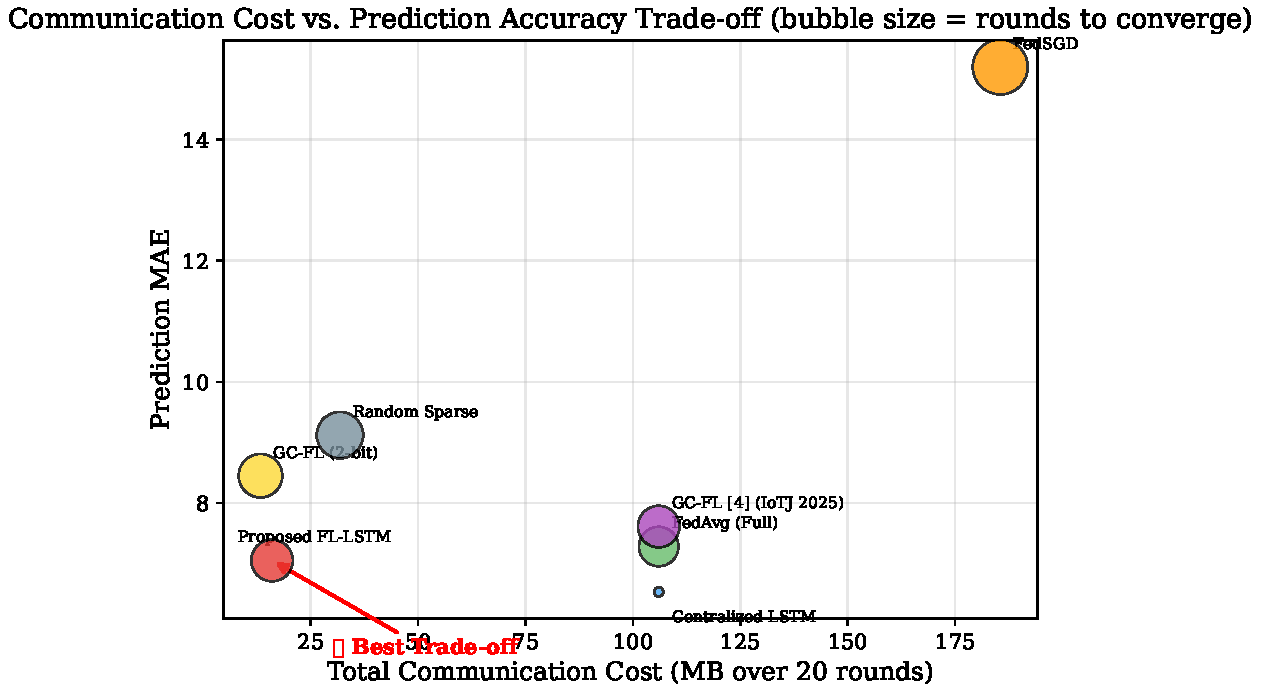
\includegraphics[width=\columnwidth]{graph12_tradeoff_analysis.pdf}
\caption{Communication cost vs. prediction accuracy Pareto analysis. FL-LSTM achieves the optimal trade-off, outperforming all baselines on the cost-efficiency ratio.}
\label{fig:graph12}
\end{figure}

\subsection{Comprehensive Performance Summary}

Table~\ref{tab:overall} provides a summary of the framework's performance across all evaluation dimensions, consolidating the comparative results from the 12 preceding analyses.

\begin{table}[!htbp]
\centering
\caption{Overall Framework Performance Summary}
\label{tab:overall}
\begin{tabular}{l c}
\toprule
\textbf{Evaluation Dimension} & \textbf{Result} \\
\midrule
\multicolumn{2}{c}{\textit{Federated Learning}} \\
Training Loss (converged) & 0.0091 \\
FL Rounds to Converge & 20 \\
Total FL Clients (Zones) & 25 \\
Model Parameters & $\sim$53,000 \\
\midrule
\multicolumn{2}{c}{\textit{Prediction Accuracy}} \\
MAE & 7.05 \\
RMSE & 13.12 \\
MAPE (filtered) & 36.94\% \\
Improvement over ARIMA & 61.7\% \\
\midrule
\multicolumn{2}{c}{\textit{Communication Efficiency}} \\
Gradient Compression Savings & 84.9\% \\
Data Transmitted (20 rounds) & 16 MB \\
Uncompressed Baseline & 106 MB \\
\midrule
\multicolumn{2}{c}{\textit{Operations}} \\
Dynamic Service Rate & 60.2\% \\
Static Service Rate (Baseline) & 46.6\% \\
Relative Improvement & 29.2\% \\
Dynamic Fleet Utilization & 56.8\% \\
Static Fleet Utilization & 33.0\% \\
Additional Rides (Dynamic) & +410 \\
\bottomrule
\end{tabular}
\end{table}



% ---------------------------------------------------------------
%      OPTIONAL SECTIONS
% ---------------------------------------------------------------

\FloatBarrier

\section*{Acknowledgment}
The authors would like to thank Vellore Institute of Technology, Chennai, for providing the computational resources and academic support for this research.

% ---------------------------------------------------------------
%      REFERENCES
% ---------------------------------------------------------------

\begin{thebibliography}{4}

\bibitem{ref1}
``Optimization of Robotaxi Dispatch With Pick-Up/Drop-Off-Point and Boarding-Time Recommendation,'' \textit{IEEE Transactions on Intelligent Transportation Systems}, 2025. [Online]. Available: \url{https://ieeexplore.ieee.org/document/11278559}

\bibitem{ref2}
``Multi-Objective Optimization for Robotaxi Dispatch With Safety-Carpooling Mode in Pandemic Era,'' \textit{IEEE Transactions on Intelligent Transportation Systems}, 2024. [Online]. Available: \url{https://ieeexplore.ieee.org/document/10745879}

\bibitem{ref3}
``Optimization of Urban Emergency Multimodal Transportation Scheduling With UAV-Ground Traffic Coordination,'' \textit{IEEE Transactions on Intelligent Transportation Systems}, vol.~27, no.~1, pp.~692--708, Jan. 2026. [Online]. Available: \url{https://ieeexplore.ieee.org/document/11235593}

\bibitem{ref4}
``Gradient Compression and Correlation-Driven Federated Learning for Wireless Traffic Prediction,'' \textit{IEEE Internet of Things Journal}, 2025. [Online]. Available: \url{https://ieeexplore.ieee.org/document/10818793}

\end{thebibliography}

% ---------------------------------------------------------------
%         APPENDICES
% ---------------------------------------------------------------

\appendix
\section{Model Architecture Details}
The LSTM traffic prediction model architecture consists of a 2-layer LSTM with 64 hidden units per layer, processing 3-feature input sequences of length 8. The output is produced through a fully connected network: $64 \rightarrow 32 \rightarrow 3$, with ReLU activation in the intermediate layer. The total trainable parameter count is approximately 53,000. Training uses the Adam optimizer with an initial learning rate of 0.001 and MSE loss. Each zone performs 3 local training epochs per FL round with a batch size of 16.

\end{document}
